\documentclass[a4paper]{article}
\usepackage[utf8]{inputenc}
\usepackage{dirtree}
\usepackage{titling}
\usepackage{minted}
\usepackage{fancyvrb}
\usepackage{graphicx}
\usepackage{float}
\usepackage[binary-units=true]{siunitx}

\graphicspath{ {images/} }

\newcommand{\subtitle}[1]{
  \posttitle{
    \par\end{center}
    \begin{center}\large#1\end{center}
    \vskip0.5em}
}
 

\title{DiSy}
\subtitle{Directory and file synchronization using Protobuf}
\author{Konstantin Lampalzer}
\date{}

\begin{document}
 
\begin{titlepage}
\maketitle
\end{titlepage}

\tableofcontents
\thispagestyle{empty}
\newpage

\section{License}
\begin{verbatim}
Boost Software License - Version 1.0 - August 17th, 2003

Permission is hereby granted, free of charge, to any person or organization
obtaining a copy of the software and accompanying documentation covered by
this license (the "Software") to use, reproduce, display, distribute,
execute, and transmit the Software, and to prepare derivative works of the
Software, and to permit third-parties to whom the Software is furnished to
do so, all subject to the following:

The copyright notices in the Software and this entire statement, including
the above license grant, this restriction and the following disclaimer,
must be included in all copies of the Software, in whole or in part, and
all derivative works of the Software, unless such copies or derivative
works are solely in the form of machine-executable object code generated by
a source language processor.

THE SOFTWARE IS PROVIDED "AS IS", WITHOUT WARRANTY OF ANY KIND, EXPRESS OR
IMPLIED, INCLUDING BUT NOT LIMITED TO THE WARRANTIES OF MERCHANTABILITY,
FITNESS FOR A PARTICULAR PURPOSE, TITLE AND NON-INFRINGEMENT. IN NO EVENT
SHALL THE COPYRIGHT HOLDERS OR ANYONE DISTRIBUTING THE SOFTWARE BE LIABLE
FOR ANY DAMAGES OR OTHER LIABILITY, WHETHER IN CONTRACT, TORT OR OTHERWISE,
ARISING FROM, OUT OF OR IN CONNECTION WITH THE SOFTWARE OR THE USE OR OTHER
DEALINGS IN THE SOFTWARE.
\end{verbatim}

\newpage

\section{Task}
Goal of the project is creating a Server-Client system used to synchronize directories and files between multiple network processes. In order to compare the files timestamps and hash values are used

\subsection{Technologies}
\texttt{DiSy} is using features introduced in the C++17 standard and therefor relies on a C++ compiler adhering to this specification. \texttt{g++} (Ubuntu 7.3.0-27ubuntu1~18.04) is used to compile \texttt{DiSy} on Ubuntu 18.04.2 LTS "bionic"..

\begin{table}[h]
\centering
\begin{tabular}{l|l}
Use-Case                      & Technology \\ \hline
Networking                    & asio       \\
Networking                    & GRPC       \\
Logging                       & spdlog     \\
Command line argument parsing & CLI11      \\
Configuration files           & json       \\
SHA-512 file hashing          & OpenSSL    \\
Data serialization            & Protobuf
\end{tabular}
\caption{Used libraries/technologies.}
\end{table}

All libraries beside OpenSSL were mandatory as by project definition. \\
OpenSSL was chosen for file hashing, because it supports SHA-512, which is deemed to be securely enough for file hashing. Additionally, it is often preinstalled on most common Linux distributions.

\subsection{Assumptions}
\begin{enumerate}
\item Only Unix-like operating systems are supported. It might work on other systems, but the software was only tested on the most recent version of Ubuntu.
\item The underlying file-system of client and server is the same $\rightarrow$
\begin{enumerate}
	\item Maximum path lengths are equal
	\item Case sensitive / insensitive paths can not be mixed
\end{enumerate}
\item All clients have working clocks that are approximately synchronized
\item Synchronization is done till a client stops the program$\rightarrow$
\begin{enumerate}
	\item Deletion of files is not included
	\item File rights are not synchronized
	\item Live editing on multiple clients is not supported
\end{enumerate}
\item Conflicts are solved server-side
\item Forced synchronization termination can result in inconsistent state
\end{enumerate}


\section{Implementation}
\subsection{Project structure}
\dirtree{%
	.1 DiSy.
	.2 build/:.
	.2 include/:.
	.3 client/:\DTcomment{All header files relevant to only the client}.
	.3 server/:\DTcomment{All header files relevant to only the server}.
	.3 shared/:\DTcomment{All header files relevant to the server and the client}.
	.4 asioNetworking.hpp:\DTcomment{Header-only. Handles all the networking done by asio}.
	.4 crawler.hpp:\DTcomment{Header-only. Responsible for crawling a directory and creating a DirTree object.}.
	.4 hashing.hpp:\DTcomment{Header-only. Takes a file and retuns the hash of this file.}.
	.4 reader.hpp:\DTcomment{Header-only. Responsible for reading files from the filesystem and turning them into a byte-array.}.
	.4 shared.hpp:\DTcomment{Header-only. General shared functions.}.
	.4 writer.hpp:\DTcomment{Header-only. Writes files from a byte-array to the filesystem.}.
	.2 src/:.
	.3 client/:.
	.4 client.cpp:\DTcomment{All general client-side functionality.}.
	.4 downloader.cpp:\DTcomment{Downloads files and directories from the server}.
	.4 main.cpp:\DTcomment{Main entrypoint for the client}.
	.4 uploader.cpp:\DTcomment{Uploads files and directories to the server}.
	.3 protos/:
	.4 DiSy.proto:\DTcomment{Proto message definition file}.
	.3 server/:
	.4 main.cpp:\DTcomment{Main entrypoint for the server}.
	.4 server.cpp:\DTcomment{All general server-side functionality.}.
	.2 meson.build:\DTcomment{}.
	.2 meson\_options.txt:\DTcomment{}.
}


\subsection{Recursive directory traversal}
The \texttt{filesystem} library was introduced into the C++ language standard in 2016. but support is still relatively poor. Still, it was decided to sacrifice support of systems without the experimental filesystem library, as it provides a hassle-free way to iterate trough all files recursively. Additionally, support will be expanded with the next C++ version, C++20.

\subsection{Protocol Buffers}
\begin{figure}[H]
\centering
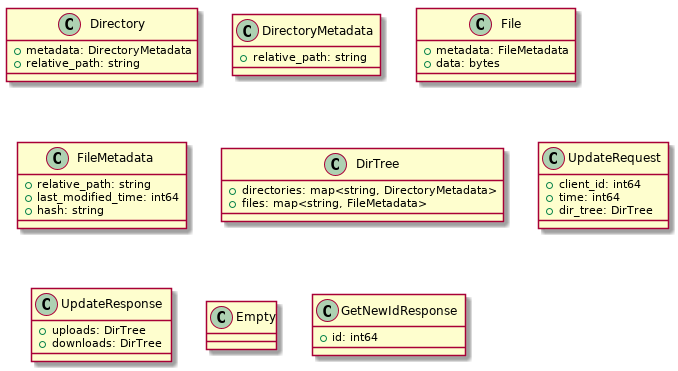
\includegraphics[height=8cm]{protobufs}
\caption{All defined Protobuf messages.}
\end{figure}

Communication between server and client is exclusively handled with Protobuf messages. 
An example of their usage in the actual protocol can be found on page~\pageref{sec:phases}.
\newpage

\subsection{Command line interface}
\begin{verbatim}
DiSy server
Usage: ./server [OPTIONS]

Options:
    -h,--help                   Print this help message and exit
    -g,--gport INT              grpc server port
    -a,--aport INT              asio server port
    -d,--dir DIR REQUIRED       Directory to synchronize
    --debug                     debug messages

--------------------------------------------------------------

DiSy client
Usage: ./client [OPTIONS]

Options:
    -h,--help                   Print this help message and exit
    -d,--dir DIR                Directory to synchronize
    -c,--config FILE            Config file
    -g,--gaddres TEXT           grpc server address
    -a,--aaddres TEXT           asio server address
    -p,--port INT               asio server port
    -debug                      debug messages
\end{verbatim}

\texttt{DiSy server} and \texttt{DiSy client} provide very similar command line interfaces. The address is not configurable for \texttt{DiSy server} because its IPv4 socket is automatically bound to 0.0.0.0.
\bigbreak
\texttt{Usage:}\\
Start the DiSy server. Then start at least two clients. They will now automatically synchronize the supplied parameters.
\bigbreak
A configuration file in the \texttt{JSON} file format can also be supplied instead of parameters on the client:

\begin{figure}[H]
\begin{minted}[]{json}
{
	"asioAddress":"0.0.0.0",
	"asioPort":8081,
	"debug":false,
	"grpcAddress":"0.0.0.0:8080",
	"path":"default"
}
\end{minted}
\caption{Example configuration file.}
\end{figure}

\section{Networking}
A slim header is perpended to Protobuf messages to determine their length and differentiate between different message types. Fixed size unsigned integers are used because their length should be identical between different operating systems and processor architectures. 

asio's \texttt{mutable\_buffer}s are used to encode all header fields before transmission.
\begin{figure}[H]
\centering
\begin{BVerbatim}
+---+------------------------+
| 1 |            8           |
+---+------------------------+
\end{BVerbatim}
\caption{Header perpended to Protobuf messages.}
\end{figure}

To cut down on boilerplate code it was decided to utilize lookup tables to dynamically determine which type of Protobuf message is being sent or received. 

\begin{figure}[H]
\begin{minted}[]{c++}
enum class MessageType
{
	FileMetadata = 1,
	File = 2
};

const std::unordered_map<std::type_index, MessageType> typeMapping{
	{typeid(DiSy::FileMetadata), MessageType::FileMetadata},
	{typeid(DiSy::File), MessageType::File}
};

\end{minted}
\caption{Shortened lookup table definition.}
\end{figure}

This decision rules out possible optimizations by the compiler, as message type lookup has to be performed at runtime. While this compromise does result in degraded performance, the difference is insignificant as most processor time will be spent waiting for file I/O operations anyways.

\begin{figure}[H]
\begin{minted}[]{cpp}
inline int sendProto(tcp::socket &socket, google::protobuf::Message &message)
{
	u_int8_t messageType{toUnderlying(typeMapping.at(typeid(message)))};
	u_int64_t messageSize{message.ByteSizeLong()};
	
	asio::write(socket, buffer(&messageType, sizeof(messageType)));
	asio::write(socket, buffer(&messageSize, sizeof(messageSize)));
	
	streambuf streamBuffer;
	ostream outputStream(&streamBuffer);
	message.SerializeToOstream(&outputStream);
	asio::write(socket, streamBuffer);
	return SEND_OK;
}
\end{minted}
\caption{Send function. All Protobuf messages are subclasses of Message, which is provided by Protobuf.}
\end{figure}

Additionally, there are two functions provided to receive the next message type and the message itself. This enables me to easily transfer any message over the network using asio. Only files are transferred over asio, everything else is communicated via gRPC.

\subsection{Protocol phases}
\label{sec:phases}
\subsubsection{First phase}
\begin{figure}[H]
\centering
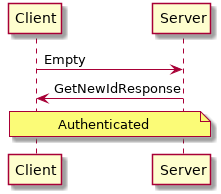
\includegraphics[width=4.5cm]{first_stage}
\caption{First phase: Client requesting an id from the server.}
\end{figure}

After the client establishes a connection to the server it requests an ID from the server. The server then creates an unique ID for the client and sends it back to the client. The client then traverses all files and directories in the specified folder to compose a \texttt{DirTree} message, which is used by the server to compute which files/directories need to be created/sent/requested.

\subsubsection{Second phase}
\begin{figure}[H]
\centering
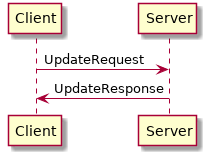
\includegraphics[width=4.5cm]{second_stage}
\caption{Second phase: Transmission of directories and files as well as requests for files that are not present on the server.}
\label{fig:stage2}
\end{figure}

After the client traversed all his local files, he creates an \texttt{UpdateRequest} message containing the current timestamp and the DirTree. The message then computes the difference between the received DirTree and the server DirTree and afterwards sends an \texttt{UpdateResponse} with all the files and directories that need to be uploaded/downloaded by the client.

\begin{figure}[H]
\begin{minted}[]{cpp}
void Client::sendUpdate()
{
	grpc::ClientContext clientContext;
	DiSy::UpdateRequest updateRequest;
	updateRequest.set_client_id(clientId);
	updateRequest.set_allocated_dir_tree(crawler::crawlDirectory(path));
	updateRequest.set_time(shared::getCurrentTime());
	
	DiSy::UpdateResponse updateResponse;
	grpc::Status status{stub->Update(&clientContext, updateRequest, &updateResponse)};
	
	uploadDirectories(updateResponse.uploads().directories());
	downloadDirectories(updateResponse.downloads().directories());
	
	uploadFiles(updateResponse.uploads().files());
	downloadFiles(updateResponse.downloads().files());
}
\end{minted}
\caption{Processing of \texttt{UpdateRequest} messages.}
\end{figure}

Directories that are present on the server but missing on the client are handled next. \texttt{DirectoryMetadata} messages are sent to the server next. For every directory request one \texttt{DirectoryMetadata} message is sent. The server responds with a Directory which is then created on the client. These steps are repeated for the FileRequests and then all the requested folders and files from the server are uploaded.

Finally, the update phase is completed and the client waits for a bit, till the update is repeated.


\subsubsection{Third phase}
\begin{figure}[H]
\centering
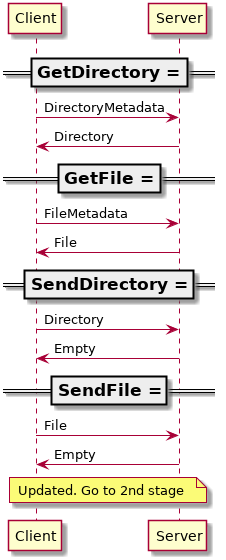
\includegraphics[width=4.5cm]{third_stage}
\caption{Third phase: Files and directories are exchanged between the server and the client.}
\end{figure}

\end{document}